%!TEX root = ../thesis.tex
\chapter{Software Architecture}
\label{chap:architecture}

In this chapter, the composition of the system is described with more detail.One of the challenges when developing SAJaS was deciding how to implement assynchronous JADE-based features in a tick-based environment. This is described in Section \ref{sec:agentexecution}. Following it is the definition of the architecture of the system in the form of conceptual diagrams. Closing this chapter is a discussion on the extension perspectives of the system.

\section{Agent Execution in SAJaS}
\label{sec:agentexecution}

% Agent execution in JADE and Repast
JADE agent execution can be concurrent and parallel, since JADE supports distributed and multi-threaded agent systems. Agent execution in Repast, on the other hand, is not concurrent. Repast uses a time-share type of execution, granting each agent the right to perform its tasks until they finish them, in sequence, but in no particular order.

% Agent execution in the API
Except when executed during their setup or takedown, agents' actions in JADE are encapsulated in Behaviours. In JADE, multiple agents can be executing their behaviours simultaneously. InRepast, however, all scheduled agents run consecutively with variable execution sequence. For the purpose of emulating a JADE-like execution more faithfully, the behaviours implemented in Repast are executed in a randomized order.

Even though a local application can take advantage of direct method invocation, when the simulation platform is single-threaded - as Repast is - there is a risk of the simulation stagnating if, for instance, two agents engage in a very long ``conversation''.

Figure \ref{fig:direct_method_execution} represents a scenario where two agents engage in a conversation that involves multiple multiple replies from both sides. With direct method invocation, the response is instantaneous but other agents don't get any time to execute in-between.

In Figure \ref{fig:assynch_execution} on the other and, each agent is allowed to execute one task - send one message, in this case. Messages stay waiting until the agent reads and processes it. This way, Agent C didn't have to wait  for the other two to finish.

\begin{figure}[ht]
	\centering
    \begin{subfigure}[b]{\linewidth}
		\centering
		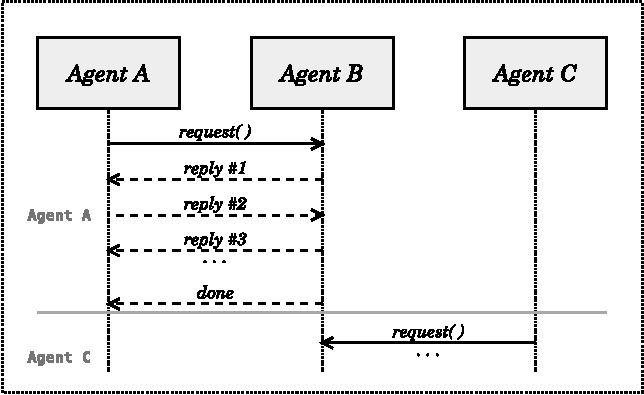
\includegraphics[width=.7\linewidth]{figures/executionProblem.pdf}
		\caption{
			With direct method invocation
		}
		\label{fig:direct_method_execution}
    \end{subfigure} \\
    \begin{subfigure}[b]{\linewidth}
		\centering
		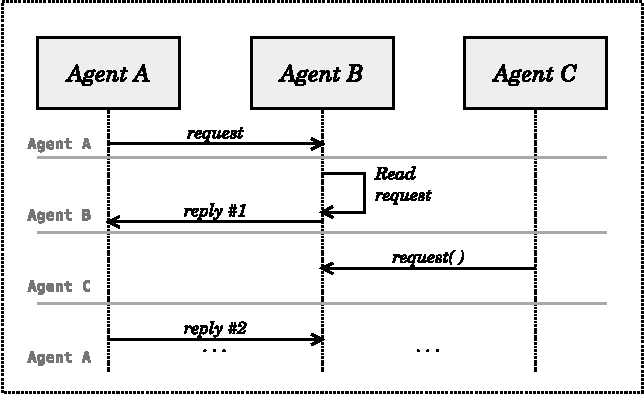
\includegraphics[width=.7\linewidth]{figures/executionProblem2.pdf}
		\caption{
			Asynchronously 
		}
		\label{fig:assynch_execution}
    \end{subfigure}
    \caption[Time sharing example]{Smaller time ``allowances'' favour fair time sharing}
    \label{fig:execution_problems}
\end{figure}

In \cite{mengistu2008scalability}, authors concluded that increasing the granularity of the system, it is possible to improve its overall performance, even if individual tasks are delayed. The granularity of an agent task is explained as the communication-to-computation, or ``a measure of the amount of computation an agent executes before entering the communication phase of one simulation time step''.

In SAJaS, as in JADE, agent interaction occurs using the available mechanism. Therefore, it asynchronous execution is appropriate for the kind of applications developed for JADE and SAJaS. To better demonstrate the differences between agent execution in both frameworks, figure \ref{fig:execution_example} and \ref{fig:com-example-repast} represent a scenario where two agents send a message to a third one who then replies. In Repast (Fig. \ref{fig:com-example-repast}), messages are delivered to agent C's message queue, and processed only in C's turn. In JADE (Fig. \ref{fig:com-example-jade}), messages can arrive concurrently. Their arrival triggers an event and they are processed right away. In this case, agent C handled the messages as they arrived and issues the respective replies.

\begin{figure}[h]
	\centering
    \begin{subfigure}[b]{\linewidth}
		\centering
		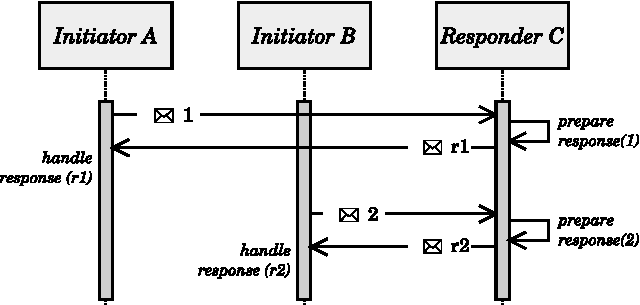
\includegraphics[width=0.7\linewidth]{figures/tickExample2.pdf}
		\caption{
			In JADE, running in parallel
		}
		\label{fig:com-example-jade}
    \end{subfigure}
    \vspace{1cm}
    \begin{subfigure}[b]{\linewidth}
		\centering
		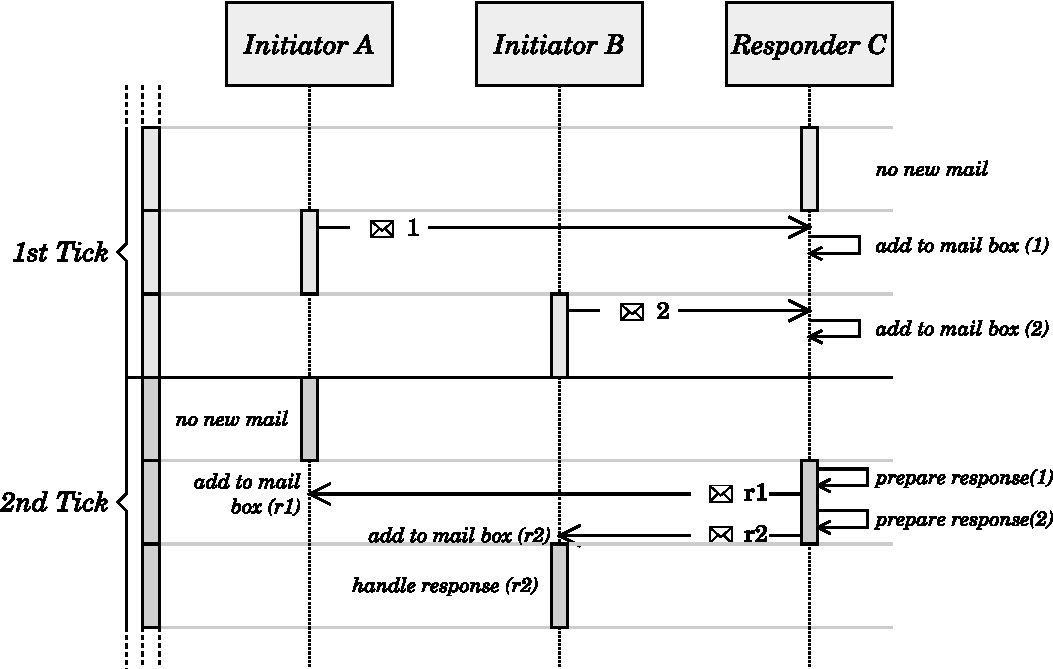
\includegraphics[width=0.9\linewidth]{figures/tickExample.pdf}
		\caption{
			In Repast, using \apiname{}.
		}
		\label{fig:com-example-repast}
    \end{subfigure}
    \caption{Communication and agent interaction}
    \label{fig:execution_example}
\end{figure}


While the diagram above represents the agents as scheduled objects, their behaviours are the ones actually being scheduled. It is worth noting that the order by which Repast executes each scheduled behaviour is unpredictable. In fact, it is not guaranteed that all the behaviours of a single agent are executed consecutively. This is the expected execution when working with Repast as well as with JADE (given its multi-threaded nature) and it is up to the programmer to ensure that the application does not rely on the order of execution.

\section{SAJaS Architecture}

From the point of view of the MAS programmer, working with this API feels the same as working with JADE, although limited to the presently available features. However, SAJaS has a much simpler internal architecture, which attempts to implement only the fundamental components needed for everything else to work. The most evident feature that was not ported from JADE was the network layer that enables the creation of distributed MAS.

Section \ref{sec:arch_conceptual} provides a broad overview of the whole system, followed by a deeper analysis of the implementation of the behaviours and protocols in Section \ref{sec:arch_behaviours}. Section \ref{sec:arch_interface} explains SAJaS' interfacing points, i.e. the way the programmer can effectively use the API.

\subsection{Conceptual Model}
\label{sec:arch_conceptual}
The diagram in Figure \ref{fig:arch} represents the internal architecture of SAJaS. The module captioned ``My Implementation'' represents an hypothetical implementation of a MAS that uses SAJaS. The ``Repast Simphony'' package's purpose is to represent dependencies of the code to Repast libraries.

Within the API, three different categories of classes are represented. First, inside the ``Repast'' package are the classes that have dependencies with Repast Simphony. Second, classes whose border is dotted are internal classes that are not meant to be used by programmers; some are not present in JADE and therefore their use cannot be ported by the conversion tool. Finally, the rest rest of the classes are the ones that programmers are expected to use and are directly supported by JADE and by the code conversion tool.

\begin{figure}[h]
	\centering
	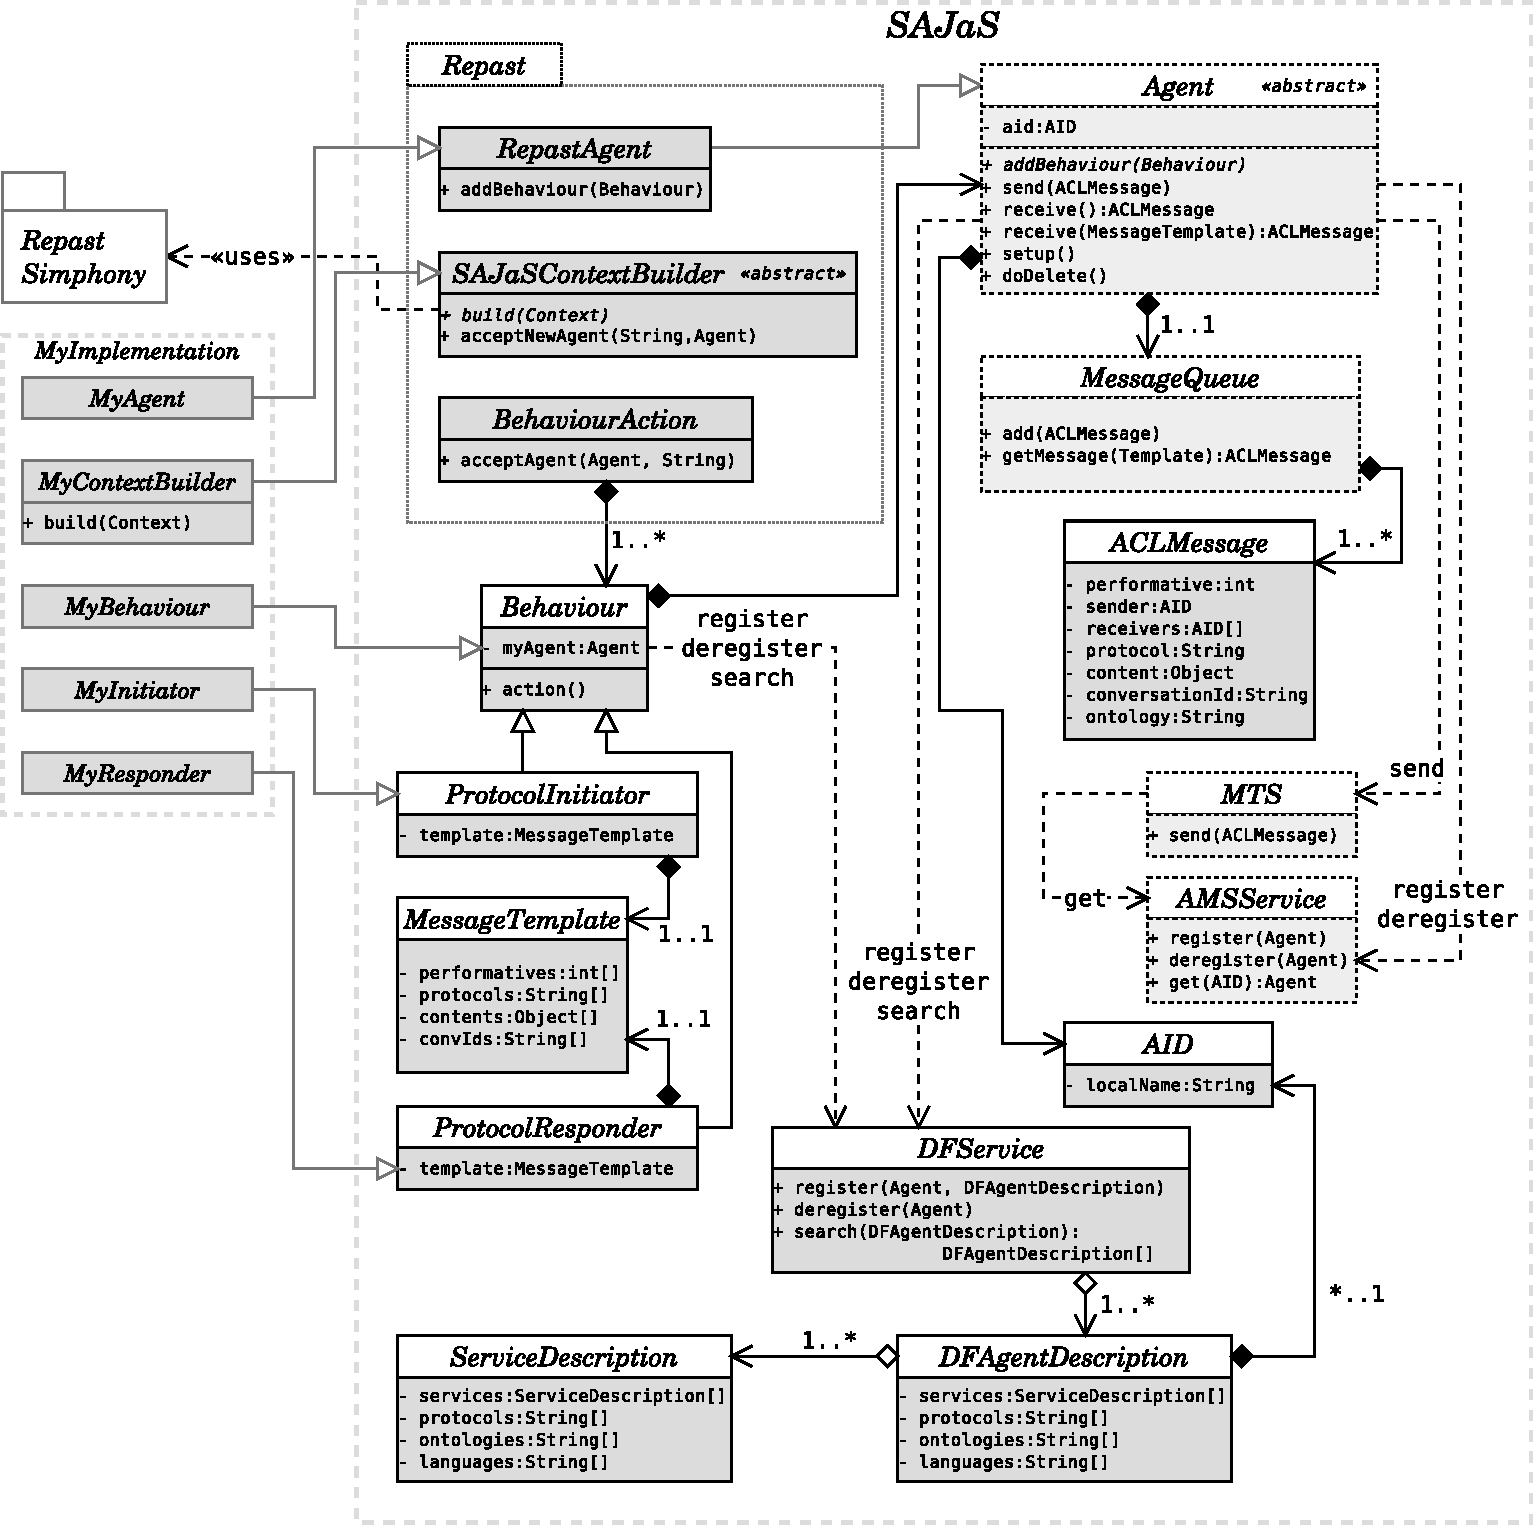
\includegraphics[width=\linewidth]{figures/sajas_arch.pdf}
	\caption[\apiname{}'s architecture]{Architecture of \apiname{}. The classes with doted border are internal.}
	\label{fig:arch}
\end{figure}

While tasks can be performed during agent setup and takedown, in runtime they are typically executed inside Behaviours. In the diagram, the Behaviour, the Protocol Initiator and the Protocol Responder are actually representations of a family of classes. For simplicity of this diagram, their complete representation is isolated in Figure \ref{fig:arch_proto}.

An agent in \apiname{} contains a MessageQueue which holds queue of ACLMessages. The Agent does not have access to its own behaviours. The behaviours, however, have access to the agent who owns them and to its MessageQueue.

The DFService, as described before, provides the yellow page service. Agents can register or deregister themselves from the DF and perform searches. The DF contains a set of DFAgentDescriptions that describe agents and the services they perform. To quickly fetch agents when a search query arrives, the DF contains a mapping of the agents that are registered with each service, protocol, ontology and language. That means that, internally, the Directory Facilitator actually contains multiple sub-directories.

Agent interaction is always established through the use of ACLMessages. At no point to agent have access to other agents. Agents use an AID to identify themselves and other Agents. Besides the Agent itself, only the AMSService knows the address corresponding to an AID.

Behaviours that implement interaction protocols contain a MessageTemplate. In the case of Finite State Machine behaviours (FSMBehaviours), this template is not fixed, but changes depending on the state of the protocol. The template is used to retrieve one message at a time from the agent's MessageQueue. One template can match multiple ACLMessages in the queue, but it always returns one single message.

\subsection{Behaviours and Protocols (Draft)}
\label{sec:arch_behaviours}
Figure \ref{fig:arch_proto} shows with higher level of detail the Behaviour module and the Protocol module. The super abstract class Behaviour has methods that are triggered by certain events. Method \texttt{action} is executed once per tick; \texttt{reset} may be called externally to reset the whole behaviour; \texttt{onEnd} is called right after the behaviour ended and was removed from the scheduler; \texttt{done} is called once per tick to determine if the behaviour ended. The default implementation of all these methods in the Behaviour class is empty and are overridden by the subclasses when needed.

The five responder initiator classes available in SAJaS implement two protocols: AchieveRE and ContractNet.

\begin{figure}
	\centering
	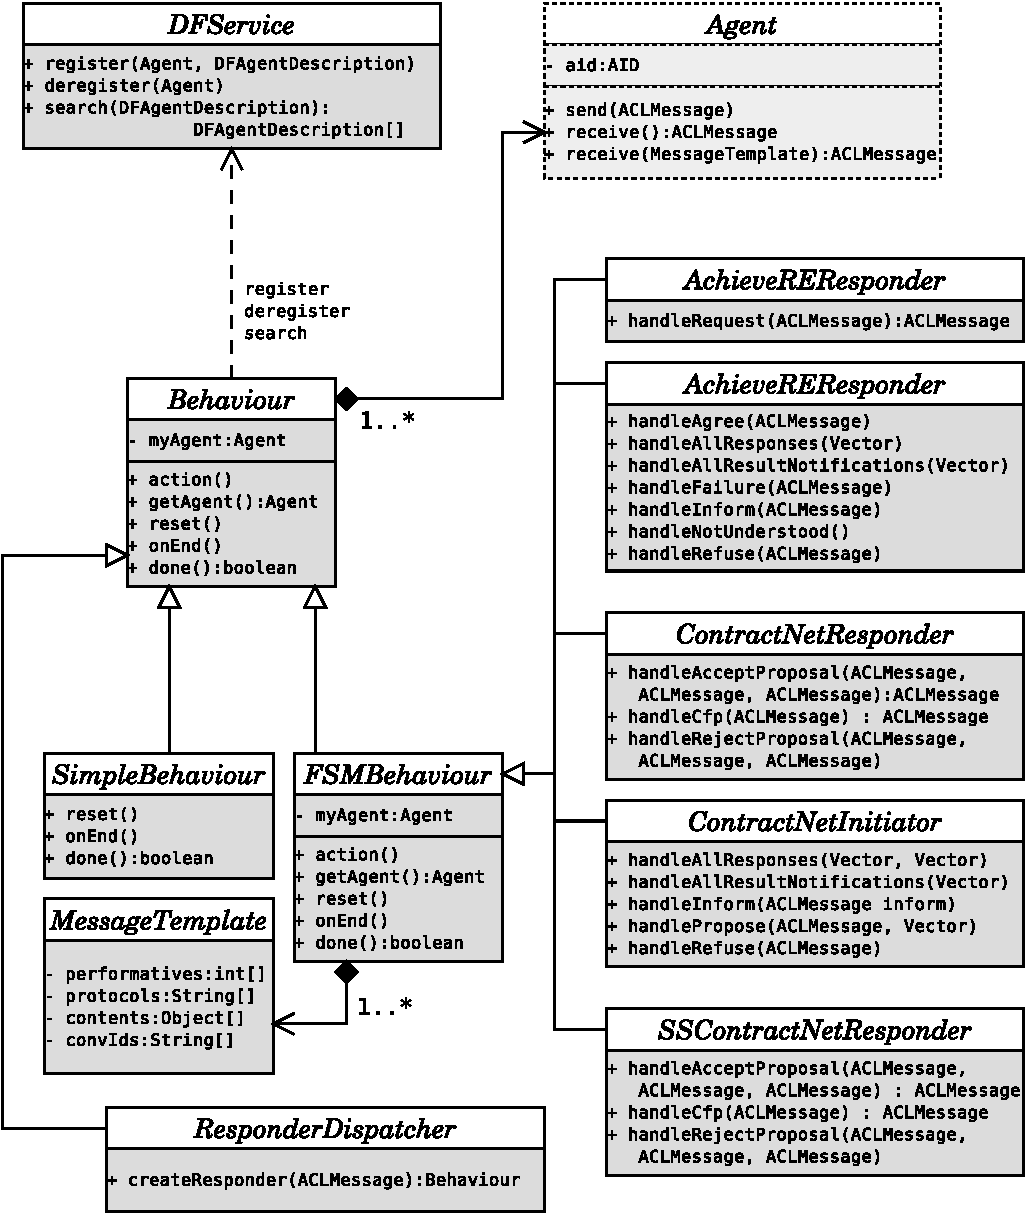
\includegraphics[width=0.7\linewidth]{figures/sajas_arch_proto.pdf}
	\caption[Behaviours and protocols in SAJaS]
	{Details of the Behaviours and Protocols in SAJaS}
	\label{fig:arch_proto}
\end{figure}

\subsection{Interfacing SAJaS (Draft)}
\label{sec:arch_interface}
The interface points of the API are the Agent, the Behaviour and their derived classes. The API also supports direct access to the DFService.

\section{Extension Perspectives (Draft)}

SAJaS was developed keeping in mind the possibility to create extensions to it's features in the future. While
this thesis was focused on providing Repast with support for FIPA standards for agent interaction (and all the infrastructure that supports it), the API is purposely generic and `framework agnostic`. Support for other simulation development tools may be added will little or no changes to the API itself.

The CCT is closely related to SAJaS, so updates to SAJaS will demand changes to the plugin as well. To facilitate the update of the plugin, it relies on a dictionary file that contains a mapping of the classes between SAJaS and JADE. The dictionary also supports some annotations that allow more that just a direct translation between two classes.


%Figure \ref{fig:arch} illustrates the details of \apiname{}'s architecture. Most concepts represented in this diagram are present in JADE, namely the Agent, ACL Message, Behaviour, MTS and DF service.
%
%An agent in \apiname{} contains a MessageQueue and a set of Behaviours. These have access to the agent who owns them and to its MessageQueue. A behaviour that implements an interaction protocol makes use of MessageTemplates. These are used to retrieve relevant messages in each step of the protocol. The MessageTemplates are updated while the protocols go through their different states.
%
%The DFService, as described before, provides the yellow page service. Agents can register or deregister themselves in the DF as well as perform searches. While tasks can be performed during agent setup, in runtime they are typically executed inside Behaviours.
%
%To follow JADE-like communication, ACL Messages carry agent identifiers (AID) for senders and receivers. These AIDs are returned by the DF as search results and are resolved to an agent by the MTS when sending a message. In \apiname{} the MTS keeps a mapping of AIDs to agents for easier access.
%
%The ``plug-in points'' of the API are the Agent, the Behaviour and their derived classes. The API also supports direct access to the DFService. In Figure \ref{fig:arch} all protocol definitions are implied by the generic sub-classes ``ProtocolInitiator'' and ``ProtocolResponder''. 
%
